\documentclass[conference]{IEEEtran}
\IEEEoverridecommandlockouts
% The preceding line is only needed to identify funding in the first footnote. If that is unneeded, please comment it out.
\usepackage{cite}
\usepackage{amsmath,amssymb,amsfonts}
\usepackage{algorithmic}
\usepackage{graphicx}
\usepackage{textcomp}
\usepackage{xcolor}
\usepackage{xspace}
\usepackage{float}
\usepackage{url}

\def\BibTeX{{\rm B\kern-.05em{\sc i\kern-.025em b}\kern-.08em
    T\kern-.1667em\lower.7ex\hbox{E}\kern-.125emX}}
\begin{document}

\title{Finding the Best Predictor of Wildfire Growth\\

}

\author{\IEEEauthorblockN{1\textsuperscript{st} Haowen Yin}
\IEEEauthorblockA{\textit{Computer Science Department} \\
\textit{Cal Poly Pomona}\\
Pomona, United States \\
hyin@cpp.edu}
\and
\IEEEauthorblockN{2\textsuperscript{nd} Dante Martinez}
\IEEEauthorblockA{\textit{Computer Science Department} \\
\textit{Cal Poly Pomona}\\
Pomona, United States \\
dantem1@cpp.edu}
\and
\IEEEauthorblockN{3\textsuperscript{rd} Wesley H. Kwan}
\IEEEauthorblockA{\textit{Computer Science Department} \\
\textit{Cal Poly Pomona}\\
Pomona, United States \\
whkwan@cpp.edu}
\and
\IEEEauthorblockN{4\textsuperscript{th} Beize Li}
\IEEEauthorblockA{\textit{Computer Science Department} \\
\textit{Cal Poly Pomona}\\
Pomona, United States \\
beizeli@cpp.edu}
}

\maketitle

\begin{abstract}
Machine learning can be used predict the size of a wildfire using regression models. The ability to accurately predict the size of a fire can serve to guide fire control and emergency evacuation measures. However, to make accurate predictions machine learning algorithms must be fed quality data. Using data collected from Montesinho Natural park, we sought to find the best predictors of wildfire growth.
\end{abstract}

\begin{IEEEkeywords}
wildfire, support vector machine, decision tree, machine learning, regression, feature selection
\end{IEEEkeywords}

\section{Introduction}
Wildfires are a serious threat to life, natural environments, and economies. From 2019 to 2020, Australia experienced unusually intense bushfires in many parts of the nation. Approximately 46 million acres were burned. Likewise in California, 2020 was a record-setting year for wildfires. It consisted of nearly 10,000 wildfires that burned more than 4.2 million acres. 

The ability to monitor and predict wildfires could further improve preventative and reactionary measures, however, monitoring wildfires presents some challenges. Challenges arise from the phenomenon's complexity. Many factors and relationships are involved in the occurrence and spread of wildfires. Such factors and relationships involve topographical and meteorological data, some of which may need to be collected in real time. To implement and represent all seemingly relevant factors in predictive models would be computationally costly and does not guarantee reliability.

Preexisting research and models have used a multitude of factors for wildfire prediction, like temperature, precipitation, relative humidity, wind speed, etc. However, as shown by authors in \cite{b2}, as low as three feature selections can produce predictive models with 97-99 percent accuracy. Using  machine learning techniques and data, our goal is to filter the relevant factors for wildfire prediction while developing a solid predictive model. The potential benefits are to provide the basic factors that should be addressed by any predictive model of wildfires growth.

% Outline: Related Work
% 1. Global transition
% 2. Authors and what they did
% 3. Explain their approach
% 4. Transition to our work
\section{Related Work}
Wildfire a common problem and a complex issue, and there are some works in this area. Younes Oulad Sayad produced a work focusing on predicting wildfire based on satellite images\cite{b2}.Sayad approaches the problem around satellite images. They build a data set based on Remote Sensing data related to the state of the crops (NDVI) and meteorological conditions (LST). Sayad's methods are Artificial Neural Network(ANN) and Support Vector Machine (SVM). The source of the data is satellite images which they considered in choosing ANN and SVM. Using these methods, Sayad's model can predict if there is a fire or not with high accuracy. We work with data on the ground, such as temperature, rain, humidity, and wind. The approach is to extract the feature with the most impact on the surrounding area.

The main work that we look at and obtain our data is from Paulo Cortez and Anibal Morais \cite{b1}. Our project is build on top of their work. They collected meteorological conditions s (e.g. temperature, wind). They used Support Vector Machine to predict small fire area. The feature they used are the primary features which are the meteorological conditions and their aim is to predict wildfire area. Our approach is to find the feature set that is the best predictor for wildfire. 

\section{Dataset}
The data was collected from the Montesinho Natural Park in Portugal from January 2000 to December 2003. There are 517 recorded samples in this data set. The data consists of values representing the Fine Fuel Moisture Code, Duff Moisture Code, Drought Code, Initial Spread index, temperature, relative humidity, wind speed, rain and area burned. Fine Fuel Moisture, Duff Moisture, Drought Code and Initial Spread Index are all values used in the Forest Fire Weather Index System. Fine Fuel Moisture Code represents the moisture levels under the shade of a forest canopy. The Duff Moisture Code and Drought Code are measurements representing the fuel for the fire. Where the DMC is the moisture levels under the uppermost decayed layer of organic matter and The DC measures dryness of the soil. Initial Spread Index is calculated from FFMC and wind values. It represents the spread potential of a fire given the current wind speed and moisture levels \cite{b3}. Area burned is the response variable and is provided in hectare.

\begin{figure}[h]
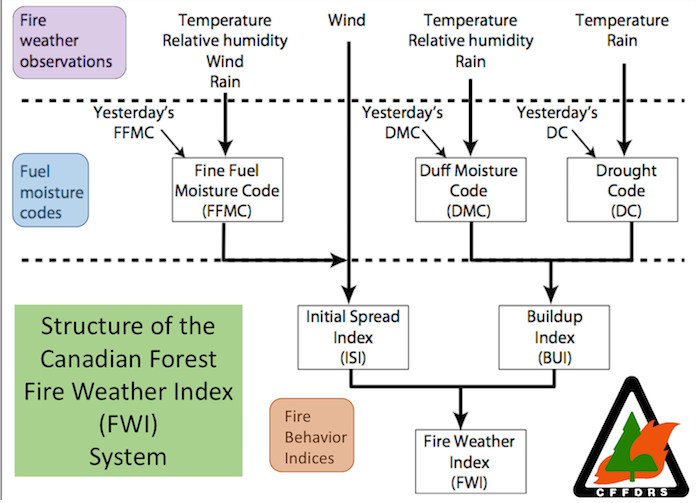
\includegraphics[width=7cm]{FireWeatherIndex.png}
\centering
\caption{The Fire Weather Index\cite{b3}}
\label{fig:Fire Weather Index}
\end{figure}

% Outline: Machine Learning model
% 1. Describe the data
% 2. State the model used
% 3. Give reasoning 
% 4. Test and record method
% 5. Conclude
\section{Machine Learning Model}
\subsection{Prediction Model}
The relevant features in our dataset are mostly numerical. Some of the features includes temperature, humidity, wind and rain. The class label is the burned area. We decided to use Support Vector Machine (SVM), and Decision Tree Regressor (DTR). The burn area should be greater than zero because zero signals very little wildfire to no wildfire. SVM should be able to separate the margin decently. The DTR algorithm ideally should organize the important features at the root. The model should split the dataset into training and test sets and perform 10-fold cross-validation. The model should be able to select features automatically and manually to test different variations. The burn area is in numerical value; hence, we shall use Mean Absolute Deviation (MAD) and Root Mean Square Error(RMSE). Both SVM and DTR perform 10 rounds of 10-fold cross-validation, and DTR's default depth will be 3.

% Outline: Feature selection
% 1. Why need feature selection
% 2. What are the ways
% 3. Explain what they are
% 4. Why we use it.
\subsection{Feature Selection}
The main idea is to find the best predictors for wildfire. We use feature selection as a means to reduce features while maintaining prediction performance. We have two processes for feature selection: feature selection algorithm and manual selection. The feature selection algorithm uses Sklearn to develop a model. Manual selection is manually selecting the feature while guided by feature correlation like Pearson, Spearman, and Kendall coefficient.
\subsubsection{Feature Selection Algorithm}
In the feature selection algorithm, f-regression and mutual information regression are used to find the relationship between the features and the target class. F-regression deals with the linear correlation between a feature and the target class. The correlation of a feature (x) and target (y) is given by the following equation:
\begin{center}
    \begin{figure}[H]
        \centering
        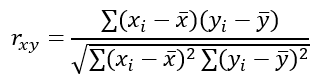
\includegraphics[width=4cm]{correlationeq.PNG}
    \end{figure}
\end{center}
The correlation value of each feature is then converted to an F score and then to a p-value. This converts the correlation of a feature and the target class to a positive value, where the larger value, the larger the relationship. Mutual information regression finds the dependency between the feature(s) and the target class. The mutual information of a feature (X) and target (Y) is given by the following equation:
\begin{center}
    \begin{figure}[H]
        \centering
        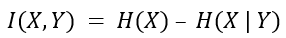
\includegraphics[width=4cm]{mutualinfoeq.PNG}
    \end{figure}
\end{center}
I(X,Y) is the mutual information of X and Y. H(X) is the entropy of X and H(X|Y) is the conditional entropy of X given Y. It quantifies the amount of information obtained about X by observing y, or vice versa. Therefore, the selected feature(s) from this algorithm are strong candidates for prediction because they have highest measurable relationship to the target.
\subsubsection{Manual Selection}
The reason to include manual selection is due to the nature of our data. Some features in our data are composite. For example, the Drought Code (DC) is a combination of temperature and rain. The algorithm can select multiple composite features that can still be vital to consider, but we will manually choose some features in the model. Manual selection cannot be based on preference; hence feature correlation should guide our decision. The three correlation coefficients we decided to use are Pearson, Spearman, and Kendall coefficients. Pearson coefficient deals with linear relationships. Spearman provides insight into the strength of a monotonic relationship. Kendall's coefficient relates to the ordinal and rank relationship. We will focus on the Pearson coefficient because it is linear, it matches F-regression in the feature selection algorithm. The following is the Pearson coefficient we used to perform manual selection.
\begin{figure}[H]
    \centering
    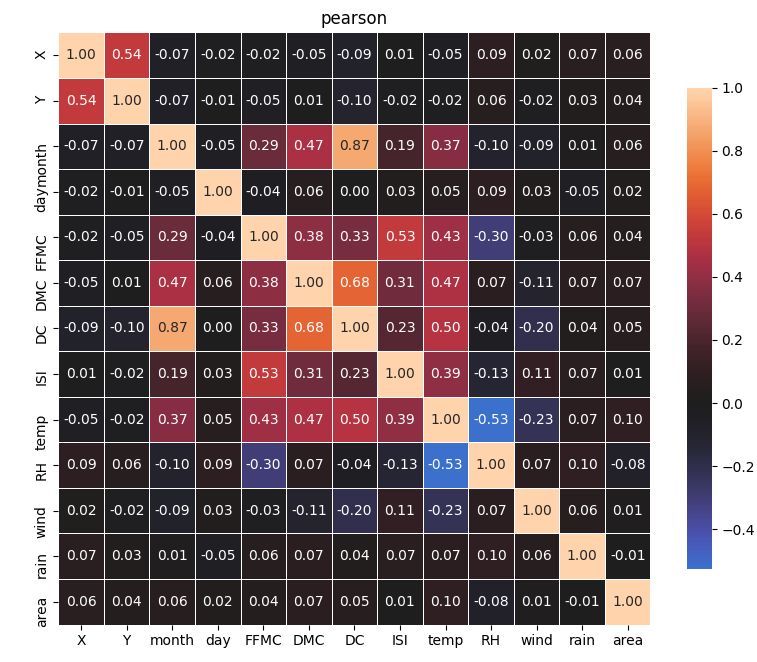
\includegraphics[width=8.5cm]{pearson.png}
    \caption{Pearson Coefficient}
    \label{fig:pearson}
\end{figure}

% Outline: Results
% 1. Baseline with no feature selection
% 2. Apply feature selection using selection algorithm
% 3. Apply manual selection
% 4. Best results 
\section{Results}
\subsection{Baseline}
First, we want to set a baseline with all features. A model that uses all features is computationally intensive. Our data is relatively small; we can run with all features and see the result before we select features. In general, a model with more features means more information, but not all features impact the prediction. 
\begin{center}
\begin{tabular}{ |c|c|c| } 
 \hline
  & SVM & DTR \\ 
 \hline
 Avg. MAD & 12.68 & 13.63 \\ 
 \hline
 Avg. RMSE & 46.43 & 46.99 \\ 
 \hline
\end{tabular}
\end{center}

\subsection{Feature Selection}
After inspecting the baseline, we want to select features that retain or surpass the baseline. First, we invoke a feature selection algorithm using f-regression and mutual information regression to compute four features. The algorithm computes the following features.

\begin{center}
\begin{tabular}{ |c|c| } 
\hline
 & Features \\ 
\hline
f-regression &  month, DMC, DC, RH\\ 
\hline
Mutual Information & month, DMC, DC, ISI\\ 
\hline
\end{tabular}
\end{center}

At this point we can run select the features and run it through SVM and DTR.
\begin{center}
    \begin{figure}[H]
        \centering
        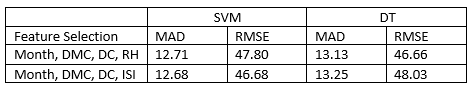
\includegraphics[width=8.5cm]{feature_selection.PNG}
        \caption{Feature Selection Algorithm Results}
        \label{fig:feature_selection_algorithm_results}
    \end{figure}
\end{center}

As we can see from the results, the value did not deviate much with four features. The SVM does perform better than DTR.

\subsection{Manual Selection}
The manual selection process is to further change the features based on the feature correlation. We made multiple selections and tested them with our model. Manual selection uses the feature selection algorithm as the baseline and performs add and drop operations on it. The Pearson coefficient guides the features that we add and drop and whether they are composite. Take the output of f-regression; it suggests using both DMC and DC features; however, these are both composite features of temperature and rain data. So, for instance, our first manual selection (in Fig. 4), we chose to drop DC and RH because they overlapped with DMC. Wind was added to the features because it had a low Pearson coefficient to both month and DMC. Given a low Pearson coefficient, the wind data had little to no correlation to either month or DMC. Two variables having high correlation means that they share some overlapping information. By selecting the one with low correlation, we can introduce more information into the model. 

\begin{center}
    \begin{figure}[H]
        \centering
        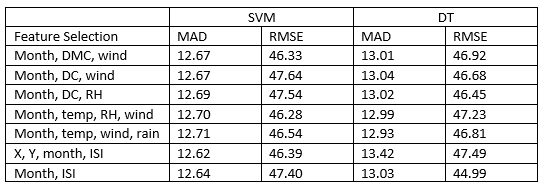
\includegraphics[width=8.5cm]{manual_selection.PNG}
        \caption{Manual Selection Results}
        \label{fig:manual_selection_results}
    \end{figure}
\end{center}

\subsection{Best Results}
From the data, we can see SVM performs better than DTR. The best MAD value is with the feature set (X,Y,month,ISI). The MAD value is too high to be considered an excellent model to predict wildfire. If we examine this feature set graphically, we can see that the prediction is mostly misplaced when the burn area increases.

\begin{center}
    \begin{figure}[H]
        \centering
        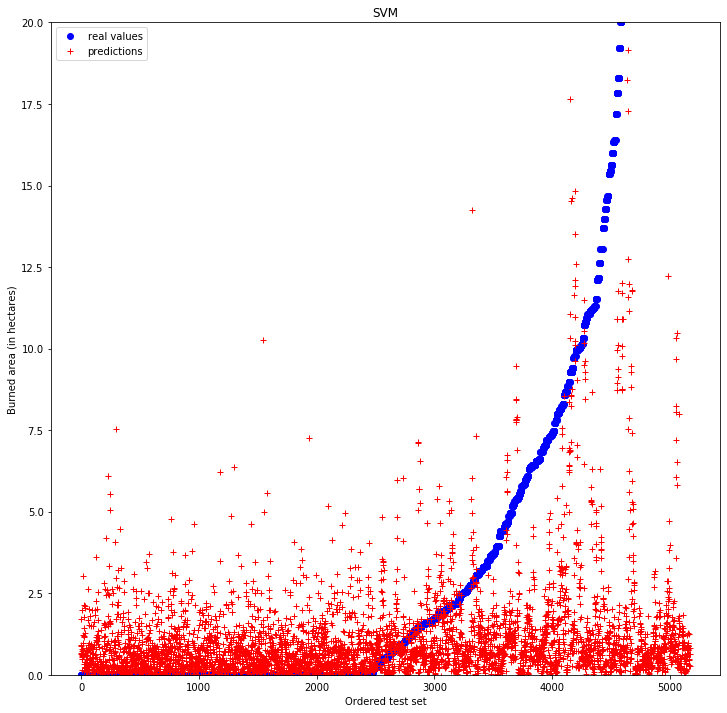
\includegraphics[width=5cm]{MAD_Best.png}
        \caption{Best MAD}
        \label{fig:best_mad_graph}
    \end{figure}
\end{center}

We can examine the one with the best RMSE. The feature set is (Month,temp,RH,wind). This feature set is more intuitive than the last one because it has three of the primary meteorological features. Once again, the graph reveals that the prediction is not on point as the burn area increases. 

\begin{center}
    \begin{figure}[H]
        \centering
        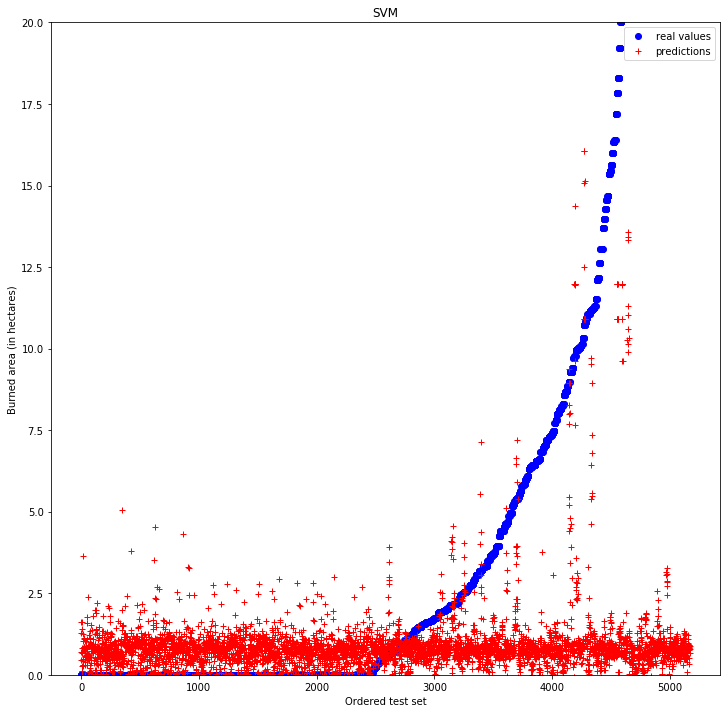
\includegraphics[width=5cm]{RMSE_Best.png}
        \caption{Best RMSE}
        \label{fig:best_RMSE_graph}
    \end{figure}
\end{center}

The feature set (Month,temp,RH,wind) fluctuates less than the feature set (X,Y,month,ISI). We consider feature set (Month,temp,RH,wind) to be the best in our results.

% Outline: Conclusion
% 1. Thesis
% 2. Describe best results
% 3. Potential error
% 4. Potential improvement

\section{Conclusion}
In conclusion, despite not developing a strong predictive model of the size of wildfires, our feature selection process and testing with our models let us determine the relevant features of the data. We mentioned how we built the feature selection algorithm using f-regression and mutual information regression to see the relationship between the features and the target class. Also, we validate our model under different conditions and lower the average MAD(Mean Absolute Deviation) and average RMSE(Root Mean Squared). The best result from both MAD and RMSE does not produce a competitive model to predict wildfire, but it can provide insight into wildfire's best predictors. The first prominent predictor is the month. It is intuitively understood that some months are vulnerable to wildfire due to environmental changes throughout the year. If we look back to our feature selection program, the two regression overlaps over two features besides the month: DMC and DC. The two features are composite features of temperature, relative humidity, and rain. The value of MAD and RMSE did not change drastically through feature selection and manual selection. The graph of the model does differ notably. The error is rooted in the data. The target class has many zero values that signal no wildfire. Zero values are difficult to deal with, primarily through regression models. There is very little improvement we can make to this dataset. When month becomes the best predictor, it signals that the features we had contained minimal information suggesting wildfire size. The features we had may correlate with wildfire, but they are not the root of what caused wildfire.

\section{Supplementary Link}
https://github.com/hyin8/CS4210\_project.git

\begin{thebibliography}{00}

\bibitem{b1} P. Cortez and A. Morais. A Data Mining Approach to Predict Forest Fires using Meteorological Data. In J. Neves, M. F. Santos and J. Machado Eds., New Trends in Artificial Intelligence, Proceedings of the 13th EPIA 2007 - Portuguese Conference on Artificial Intelligence, December, Guimarães, Portugal, pp. 512-523, 2007. APPIA, ISBN-13 978-989-95618-0-9. http://www3.dsi.uminho.pt/pcortez/fires.pdf

\bibitem{b2} Sayad, Y., Mousannif, H. and Al Moatassime, H., 2021. Predictive modeling of wildfires: A new dataset and machine learning approach. https://www.sciencedirect.com/science/article/abs/pii/S0379711218303941

\bibitem{b3} “Fire weather Index (fwi) system,” 10-Mar-2021. [Online]. Available: https://www.nwcg.gov/publications/pms437/cffdrs/fire-weather-index-system. [Accessed: 25-Mar-2021]. 

\bibitem{b4}{W. Badr, “Why Feature Correlation Matters .... A Lot!,” Medium, 22-Jan-2019. [Online]. Available: https://towardsdatascience.com/why-feature-correlation-matters-a-lot-847e8ba439c4. [Accessed: 12-May-2021].}
\end{thebibliography}

\end{document}
